\documentclass[12pt]{beamer}
\usefonttheme{serif}
\usepackage[utf8]{inputenc}
\usepackage[T1]{fontenc}
\usepackage{graphicx}
\usepackage{amsmath}
\usepackage{lmodern}
\usepackage{tikz}
\usepackage[ngerman]{babel}
\usepackage{csquotes}
\usetikzlibrary{positioning, arrows.meta, shapes.geometric, backgrounds}
\usetheme{Madrid}
\setbeamertemplate{caption}[numbered]
\begin{document}
	\author{Wilfried Keller}
	\title[DeepSurvival \& Support]{Wirksamkeitsanalyse von Hochschulsupport und Prognose des Studienverlaufs}
	\subtitle{Abschlussprojekt im Kurs: \emph{Deep Learning}\\ bei \textbf{Dr. Bernd Ebenhoch}}
	\institute[alfatraining]{alfatraining Bildungszentrum}
	\date{31.07.2026}
	\subject{DeepLearning}
	\setbeamertemplate{navigation symbols}{}

\begin{frame}[plain]
	\maketitle
\end{frame}

\begin{frame}{Motivation \& Vorgeschichte}
    \begin{itemize}
        \item \textbf{Der Auslöser:} Vorher habe ich selbst (im Team) an der HSKL einen hybriden Mathe-Support entwickelt und mich gefragt: \emph{Was genau bringt das? Und wie würde ich die Wirkung \emph{datengetrieben} prüfen?}
        \item \textbf{DE:} Erste Konzeption von Datenstrukturen (ER-Modelle) und Simulation per SQL.
        \item \textbf{DA:} Aufbau einer dynamisch-stochastischen Python-Simulation.
        \begin{itemize}
            \item Untersuchung mittels \textit{Survival-Analyse} und \textit{Cox-Regression}.
            \item Visualisierung in Dashboards.
        \end{itemize}
        \item \textbf{Deep Learning (Aktuelles Projekt):} Erweiterung der Thematik um Techniken des Maschinellen und Deep Learnings: \emph{Was wird besser?}
    \end{itemize}
\end{frame}

\begin{frame}{Exkurs: Grundlagen der Survival-Analyse}
    \footnotesize
    \textbf{Warum nicht einfach logistische Regression?}
    \begin{itemize}
        \item \textbf{Zensierung:} Wir wissen oft nur: \enquote{Bis Semester X noch kein Abbruch}.
        \item \textbf{Zeitkomponente:} Es geht nicht nur darum \textit{ob}, sondern \textit{wann} Dropout eintritt.
    \end{itemize}
    \textbf{Zentrale Begriffe}
    \begin{itemize}
        \item \textbf{Survival-Funktion $S(t)$:} Überlebenswahrscheinlichkeit bis Zeit $t$ (z.B. Kaplan-Meier).
        \item \textbf{Hazard-Rate $h(t)$:} Momentanes Risiko zum Zeitpunkt $t$.
        \item \textbf{Hazard Ratio (HR):} Relatives Risiko. \emph{HR < 1 bedeutet Risikosenkung (positiv).}
    \end{itemize}
    \vspace{-0.3cm}
    \begin{center}
        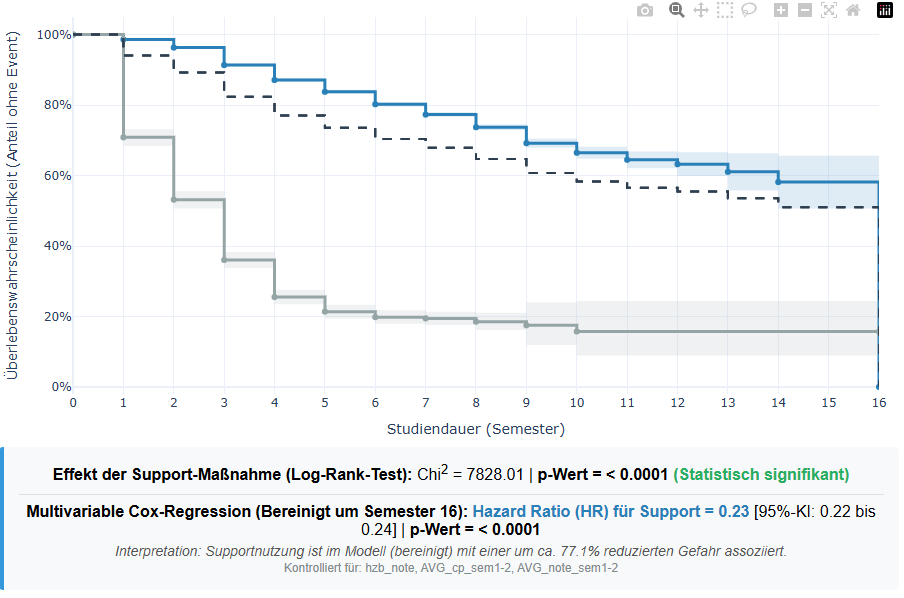
\includegraphics[height=0.32\textheight,keepaspectratio]{../output_dl/plots/dashboard_screenshot.png}
    \end{center}
\end{frame}

\begin{frame}{Setup: Makro-Struktur der Simulation}
Die Simulation ist ein dynamisches Modell (mit Feedbackschleifen und daher Nicht-Linearität -- und jeder Menge Rauschen)!
    \centering
    \scalebox{0.75}{
    \begin{tikzpicture}[
        >=Latex,
        box/.style={draw, rectangle, rounded corners, align=center, fill=blue!5, text width=2.4cm, font=\scriptsize, inner sep=4pt},
        latent/.style={draw, rectangle, rounded corners, align=center, fill=yellow!10, text width=2.4cm, font=\scriptsize, inner sep=4pt},
        action/.style={draw, ellipse, align=center, fill=orange!10, font=\scriptsize, inner sep=2pt, text width=2cm},
        outcome/.style={draw, rectangle, rounded corners, align=center, fill=red!10, text width=2.4cm, font=\scriptsize, inner sep=4pt}
    ]
    
    % --- Spalte 1: Inputs ---
    \node[box, fill=gray!10] (hzb) at (0, 3) {HZB-Note \&\\Demografie};
    \node[box, fill=gray!10] (erwerb) at (0, -1.5) {Erwerbstätigkeit\\(h/Woche)};
    
    % --- Spalte 2: Dynamische Zustände & Zeitbudget ---
    \node[latent] (erwartung) at (4, 4.5) {Erwartete Note\\(Fähigkeiten)};
    \node[latent] (motivation) at (4, 3) {Motivation};
    \node[latent] (integration) at (4, 1.5) {Soz. Integration};
    
    % Nested Zeitbudget
    \node[box, fill=cyan!10, fill opacity=0.4, text opacity=1, minimum height=1.6cm, minimum width=3.4cm] (budget_bg) at (4, -1.5) {};
    \node[font=\scriptsize, align=center, anchor=north] (budgetlabel) at (budget_bg.north) {Zeitbudget};
    \node[box, fill=red!10, text width=2.6cm, inner sep=2pt] (overload) at (4, -1.8) {Overload-Penalty};
    
    % --- Spalte 3: Aktionen & CP-Konto ---
    \node[action] (support) at (8, 4.5) {Supportnutzung};
    \node[action] (module) at (8, 2.5) {Modulwahl\\(Workload)};
    
    % Nested CP-Konto
    \node[box, fill=cyan!10, fill opacity=0.4, text opacity=1, minimum height=1.6cm, minimum width=3.4cm] (cpkonto_bg) at (8, 0) {};
    \node[font=\scriptsize, align=center, anchor=north] (cplabel) at (cpkonto_bg.north) {CP-Konto};
    \node[box, fill=red!10, text width=2.6cm, inner sep=2pt] (cprisk) at (8, -0.3) {CP-Rückstand};
    
    % --- Spalte 4: Exits ---
    \node[outcome, fill=green!20] (abschluss) at (12.5, 4.5) {Abschluss\\(180 CP)};
    
    % Nested Prüfungsleistung
    \node[box, fill=gray!20, fill opacity=0.4, text opacity=1, minimum height=1.6cm, minimum width=3.4cm] (leistung_bg) at (12.5, 2.2) {};
    \node[font=\scriptsize, align=center, anchor=north] (leistung_label) at (leistung_bg.north) {Prüfungsleistung};
    \node[box, fill=green!20, text width=1.2cm, inner sep=2pt] (pass) at (11.7, 1.8) {Pass};
    \node[box, fill=red!20, text width=1.2cm, inner sep=2pt] (fail) at (13.3, 1.8) {Fail};
    
    \node[outcome, fill=red!20] (dropout) at (12.5, -1.5) {Dropout-Risiko\\(Studienabbruch)};
    
    % --- Edges: Initial Setup ---
    \begin{scope}[on background layer]
    \draw[->, thick, gray] (hzb.east) to[out=0, in=180] (erwartung.west);
    \draw[->, thick, gray] (hzb.east) to[out=0, in=180] (motivation.west);
    \draw[->, thick, gray] (hzb.east) to[out=0, in=180] (integration.west);
    \draw[->, thick, gray] (erwerb.east) -- (budget_bg.west);
    
    % --- Edges: Actions & Budgets ---
    \draw[->, thick, gray] (erwartung.east) -- (support.west);
    \draw[->, thick, gray] (motivation.east) to[out=0, in=180] (support.west);
    \draw[->, thick, gray] (integration.east) to[out=0, in=210] (support.south west);
    
    \draw[->, thick, gray] (budget_bg.east) to[out=0, in=225] (module.south west);
    
    % Time Costs (Red arrows going backwards/downwards)
    \draw[->, thick, red] (module.south west) to[out=225, in=45] (budget_bg.north east);
    \draw[->, thick, red] (support.south west) to[out=225, in=90] (budget_bg.north);
    
    \draw[->, thick, green!60!black] (cpkonto_bg.north) to[out=90, in=270] (abschluss.south);
    
    % --- Edges: Leistung ---
    \draw[->, thick, green!60!black] (support.east) to[out=0, in=135] (leistung_bg.north west);
    \draw[->, thick, gray] (module.east) -- (leistung_bg.west);
    \draw[->, thick, gray] (erwartung.east) to[out=0, in=150] (leistung_bg.north west);
    \draw[->, thick, gray] (motivation.east) to[out=0, in=180] (leistung_bg.west);
    \draw[->, thick, gray] (integration.east) to[out=0, in=210] (leistung_bg.south west);
    \draw[->, thick, red] (overload.east) to[out=0, in=270] (fail.south);
    
    % --- Edges: Dropout ---
    \draw[->, thick, red] (fail.south) to[out=270, in=90] (dropout.north);
    \draw[->, thick, red] (cprisk.east) to[out=0, in=150] (dropout.north west);
    \draw[->, thick, red] (overload.east) to[out=0, in=180] (dropout.west);
    \draw[->, thick, red] (motivation.east) to[out=0, in=150] (dropout.north west);
    \draw[->, thick, red] (integration.east) to[out=0, in=180] (dropout.west);
    
    % --- Feedback Loops (Dashed) ---
    \draw[->, thick, dashed, green!60!black] (pass.south) to[out=270, in=0] (cpkonto_bg.east);
    \draw[->, thick, dashed, violet] (leistung_bg.north) to[out=90, in=0] (erwartung.east);
    \draw[->, thick, dashed, red] (fail.south west) to[out=225, in=-45] (motivation.south east);
    \end{scope}
    
    \end{tikzpicture}
    }
\end{frame}

\begin{frame}{Selektionsbias und Störfaktoren}
Eine naive Analyse der Daten zeigt: Studierende, die Support nutzen, haben einen schlechteren Notenschnitt und eine längere Studiendauer als Studierende, die keinen Support nutzen.\\
    \vspace{0.3cm}
\emph{Schadet Support sogar?}    
    \begin{itemize}
        \item \textbf{Das Dropout-Paradoxon:} Studierende, die Supportangebote intensiv nutzen, haben in unkontrollierten, statischen Modellen oft ein \textit{höheres} Dropout-Risiko.
        \vspace{0.2cm}
        \item \textbf{Die Ursache: (time-varying) Confounding:}
        \begin{itemize}
	\item Supportnutzung ist selektiv: Schwächere Studierende brauchen mehr Support
            \item Supportnutzung wird oft reaktiv ausgelöst (z.B. nach einer schlechten Note, insbesondere nach einem Fehlversuch).
            \item Die schlechte Note ist ein Indikator für ein bereits erhöhtes Risiko.
%            \item \textit{Statische Modelle (z.B. klassisches Cox-PH) können diese Pfadabhängigkeit nicht adäquat auflösen.}
        \end{itemize}
   %     \vspace{0.2cm}
   %     \item \textbf{Die methodische Hürde:} Die Support-Intervention verändert \textit{zukünftige} Zustände (Motivation, CP-Rückstand), welche wiederum \textit{zukünftige} Supportnutzung und Dropout-Wahrscheinlichkeiten beeinflussen (Feedback Loop).
    \end{itemize}
\end{frame}

\begin{frame}{Statischer vs. Dynamischer Confounder}
    \begin{columns}[T]
        
        % Linke Spalte: Das alte statische Setup
        \begin{column}{0.48\textwidth}
            \textbf{1. Statisches Setup} \\[1em]
            \centering
            \scalebox{0.9}{
            \begin{tikzpicture}[
                >=Latex,
                box/.style={draw, rectangle, rounded corners, align=center, fill=blue!10, text width=1.5cm, font=\tiny, inner sep=2pt},
                exitred/.style={draw, rectangle, rounded corners, align=center, fill=red!20, text width=1.3cm, font=\tiny, inner sep=2pt},
                exitgreen/.style={draw, rectangle, rounded corners, align=center, fill=green!20, text width=1.3cm, font=\tiny, inner sep=2pt}
            ]
            % Nodes (Rauten-Anordnung)
            \node[box, fill=gray!20] (hzb) at (1.5, 2.2) {HZB-Note\\(statisch)};
            \node[box] (support) at (0, 1) {Fachl. Support};
            \node[box] (leistung) at (3, 1) {Leistung};
            \node[exitgreen] (abschluss) at (0.5, -0.4) {Abschluss};
            \node[exitred] (abbruch) at (2.5, -0.4) {Abbruch};
            
            % Edges
            \draw[->, thick, gray] (hzb) -- (support);
            \draw[->, thick, gray] (hzb) -- (leistung);
            \draw[->, thick, green!70!black] (support) -- node[below, font=\tiny] {wirkt auf (+)} (leistung);
            \draw[->, thick, gray] (leistung) -- (abbruch);
            \draw[->, thick, gray] (leistung) -- (abschluss);
            \end{tikzpicture}
            }
            
            \vspace{0.3cm}
            \scriptsize
            \begin{itemize}
                \item HZB-Note war der primäre (statische) Störfaktor.
                \item Leicht durch einfache Cox-Regression mit Kontrollvariablen zu kontrollieren.
            \end{itemize}
        \end{column}
        
        % Rechte Spalte: Das neue dynamische Setup
        \begin{column}{0.5\textwidth}
            \textbf{2. Dynamisches Setup} \\[1em]
            \centering
            \scalebox{0.9}{
            \begin{tikzpicture}[
                >=Latex,
                box/.style={draw, rectangle, rounded corners, align=center, fill=blue!10, text width=1.6cm, font=\tiny, inner sep=2pt},
                confounder/.style={draw, rectangle, rounded corners, align=center, fill=red!10, dashed, thick, text width=1.6cm, font=\tiny, inner sep=2pt},
                exitred/.style={draw, rectangle, rounded corners, align=center, fill=red!20, text width=1.3cm, font=\tiny, inner sep=2pt},
                exitgreen/.style={draw, rectangle, rounded corners, align=center, fill=green!20, text width=1.3cm, font=\tiny, inner sep=2pt}
            ]
            % Nodes (Rauten-Anordnung)
            \node[confounder] (fails) at (1.5, 2.2) {Verg. Fehlversuche};
            \node[box] (support) at (0, 1) {Support ($t$)};
            \node[box] (leistung) at (3, 1) {Leistung ($t+1$)};
            \node[exitgreen] (abschluss) at (0.5, -0.4) {Abschluss};
            \node[exitred] (abbruch) at (2.5, -0.4) {Abbruch};
            
            % Edges
            \draw[->, thick, green!70!black] (fails) -- node[left, font=\tiny] {erhöht (+)} (support);
            \draw[->, thick, red] (fails) -- node[right, font=\tiny] {senkt (-)} (leistung);
            \draw[->, thick, green!70!black] (support) -- node[below, font=\tiny] {verbessert (+)} (leistung);
            \draw[->, thick, gray] (leistung) -- (abbruch);
            \draw[->, thick, gray] (leistung) -- (abschluss);
            \end{tikzpicture}
            }
            
            \vspace{0.3cm}
            \scriptsize
            \begin{itemize}
                \item \textbf{Das Problem:} Fehlversuche sind ein \textit{zeitveränderlicher} Confounder.
                \item Frust triggert Support-Nutzung und verschlechtert gleichzeitig Folgeleistungen.
            \end{itemize}
        \end{column}
    \end{columns}
    \vspace{0.4cm}
    \begin{center}
    \textbf{Konsequenz (Vorgriff):} \\
    \emph{Statisches Modell:} HR $> 1.0$ (Support schadet scheinbar) $\longrightarrow$ \emph{Dynamisches Modell:} HR $\approx 0.37$ (sehr deutlicher \enquote{Effekt})
    \end{center}
\end{frame}

\begin{frame}{Die Lösung: Deep Survival Analysis}
    \footnotesize
    \textbf{Ansatz: Längsschnitt-Modelle \& Neuronale Netze}
    \vspace{0.05cm}
    
    \begin{itemize}
        \item \textbf{DeepSurv \& Extended Cox:} Daten im Panel-Format $\rightarrow$ zeitveränderliche Kovariaten in jedem Semester-Schritt modellierbar.
        \vspace{0.05cm}
        \item \textbf{Recurrent \& Transformer Survival:}
        \begin{itemize}
            \item Inspiriert von DeepSurv++ / DeepHit: LSTM-/GRU- und Transformer-Architekturen kodieren die gesamte Historie in dynamische \textit{Hidden States}.
            \item \textit{Achtung:} Exzellent in der Prognose, aber für isolierte kausale HR-Schätzung aufgrund mangelnder Generalisierung problematisch.
        \end{itemize}
        \vspace{0.05cm}
        \item \textbf{Ergebnis (Isolierung des Effekts):} 
        \begin{itemize}
            \item Kontrolle vergangener Fehlversuche lässt die scheinbar negative Korrelation verschwinden.
            \item In geeigneten Panel-Modellen wird der isolierte \textit{positive} Effekt messbar.
        \end{itemize}
    \end{itemize}
\end{frame}

\begin{frame}{Methodenvergleich: Survival-Modelle (Wirkung)}
    \vspace{0.2cm}
    \begin{table}[]
        \centering
        \resizebox{\textwidth}{!}{
        \renewcommand{\arraystretch}{1.5}
        \begin{tabular}{lllp{6cm}}
            \hline
            \textbf{Modell} & \textbf{Datenstruktur} & \textbf{Confounder-Kontrolle} & \textbf{Hazard Ratio (Support)} \\ \hline
            \textbf{Landmark Cox} & 2D Snapshot & Statisch & HR $> 1$ (Verzerrt: Selektionsbias) \\
            \textbf{DeepSurv} & 2D Snapshot & Statisch (Non-linear) & HR $> 1$ (Verzerrt: Selektionsbias) \\
            \textbf{Extended Cox} & Panel (Zeitreihe) & Dynamisch (Zeitveränderlich) & \textbf{HR $\approx 0.37$} (Entstörter Effekt) \\
            \textbf{Extended DeepSurv} & Panel (Zeitreihe) & Dynamisch (Non-linear) & \textbf{HR $\approx 0.88$} \textit{(Via kontrafaktischer Simulation)} \\ \hline
        \end{tabular}
        }
    \end{table}
    
\textbf{Zwischenfazit:}
    \begin{itemize}
        \item Um \enquote{Kausalität} und echte Hazard Ratios (HR) zu messen, sind interpretierbare Panel-Modelle (Extended Cox) unerlässlich. 
	\item Die komplexeren rekurrenten Modelle eignen sich für diese spezifische HR-Analyse \textit{nicht}; auf Prognose ausgelegte Modelle naiv für kontrafaktisch Vorhersage zu verwenden scheiterte im Kurztest dramatisch ($HR > 1,5$)
    \end{itemize}
\end{frame}

\begin{frame}{Prognose \& Früherkennung (Operativer Einsatz)}
    \footnotesize
    \emph{Perspektivenwechsel: Für ein operatives Frühwarnsystem brauchen wir keine Kausalität – nur exzellente Prognosen. Welches Modell wäre geeignet?}
    \vspace{0.1cm}
    
    \begin{table}[]
        \centering
        \resizebox{\textwidth}{!}{
        \renewcommand{\arraystretch}{1.5}
        \begin{tabular}{lllp{6cm}}
            \hline
            \textbf{Aufgabe} & \textbf{Modell} & \textbf{Metriken} & \textbf{Erkenntnis} \\ \hline
            \textbf{Regression} & Keras MLP (Baseline) & $R^2 \approx 0.89$ & Target-Leakage behoben. \\
            \textbf{Regression} & LSTM (Semester) & $R^2 \approx 0.93$ &  \textbf{Trotzdem hohe Werte}: Simulations-Artefakt \\
            \textbf{Regression} & GRU (Prüfung) & $R^2 \approx 0.92$ & (CP/Fehlversuche sind wohl ein guter Notenproxy) \\
            \textbf{Klassifikation} & DeepHit & ROC: 0.83 $|$ PR: 0.28 & Multi-Task Modellierung funktioniert sehr gut. \\
            \textbf{Klassifikation} & Transformer (causal masked) & ROC: 0.82 $|$ PR: 0.29 & Attention ist stark (Baserate 2-5\% $\rightarrow$ \textbf{$\sim$10x Lift!}) \\
            \textbf{Klassifikation} & GRU (Prüfung) & ROC: 0.90 $|$ PR: 0.25 & Erkennt Dropout-Muster (Fails, CP-Verlauf) präzise. \\ \hline
        \end{tabular}
        }
    \end{table}
    \vspace{0.1cm}
    \footnotesize
    \begin{itemize}
        \item \textbf{Fazit:} Ein $R^2 > 0.90$ ist hier \emph{auch} als \textbf{Simulations-Artefakt} zu sehen: CP, Fails und Note entstehen aus derselben latenten \enquote{Fähigkeit}.
        \item In echten Daten wäre das Rauschen bei der Regression deutlich höher, während die \textbf{Klassifikation zur Frühwarnung robuster} bleibt.
    \end{itemize}
\end{frame}

\begin{frame}{Fazit}
    \footnotesize
    \begin{itemize}
        \item \textbf{Die Methodik ist entscheidend:} 
        \begin{itemize}
            \item Naive statische Analysen führen zu falschen Schlüssen.
            \item Komplexe Bildungsverläufe erfordern longitudinale Datenstrukturen.
        \end{itemize}
        \item \textbf{Trade-Off zwischen Modellen:}
        \begin{itemize}
            \item \textit{Extended Cox} für validen Wirkungsnachweis und Erklärbarkeit.
            \item \textit{Deep Sequence Models} als starke Engine für operative Frühwarnsysteme.
        \end{itemize}
        \item \textbf{Neuronale Netze sind keine Magie:}
        \begin{itemize}
            \item PH-Annahmen \& Linearität werden aufgegeben -- bezahlt mit schlechter Extrapolation auf ungesehene Muster.
            \item \textit{Eigene Versuche:} Kontrafaktischer Dauer-Support $\Rightarrow$ $HR > 1{,}5$ -- Generalisierung scheitert.
        \end{itemize}
    \end{itemize}
\end{frame}

\begin{frame}{Ausblick \& Future Work}
    \small
    \textbf{Kausale Inference \& Kontrafaktische Modelle}
    \vspace{0.15cm}
    
    \begin{itemize}
        \item \textbf{Echte Kausalität} geht aus den Beobachtungsdaten nicht abschließend hervor (ungemessene Faktoren bleiben).
        \vspace{0.1cm}
        \item \textbf{PyTorch / PyCox Refactor:} 
        \begin{itemize}
            \item Evaluierung von Modellen mit explizitem Treatment-Effekt-Kopf, die ITE unter Ignorability-Annahme direkt schätzen.
	\item Marginal Structural Models für kontrafaktische Modellierung adaptieren.
        \end{itemize}
        \vspace{0.1cm}
        \item \textbf{Beziehung zu rekurrenten Modellen ausbauen:}
        \begin{itemize}
            \item Wie können wir die gute Prädiktionskraft der Transformer/GRUs nutzen, ohne bei kontrafaktischen Was-wäre-wenn-Szenarien an der schlechten Generalisierung zu scheitern? 
        \end{itemize}
    \end{itemize}
\end{frame}

\end{document}